\chapter{Foundation Models in High Energy Physics}
\label{ch:foundation_models}

One of the main driving forces behind the successes and widespread adoption of machine learning in NLP and CV is the utilization of large pre-trained models, often referred to as foundation models (FMs)~\cite{OpportunitiesRisksFoundation}.
Especially for language tasks, most modern applications are built on top of publicly available \textit{pre-trained} FMs, such as BERT~\cite{BERT} or GPT~\cite{GPT, GPT2}, which already possess a basic understanding of language.
FMs are large models typically trained on a large corpus of domain-related data to learn expressive but generic representations of the subject.
This pre-training step is designed to be non-task-specific and is usually self-supervised (SSL), after which FMs may be \textit{fine-tuned} on specific \textit{downstream} tasks.

This system of SSL pre-training followed by supervised fine-tuning is prevalent in the many FMs in NLP~\cite{BERT, GPT, GPT2, BART, LanguageModelsAre} and CV~\cite{DINO, Dalle, Flamingo, MAE, BEIT, IJepa}.
Current research in these fields is focused on developing new SSL strategies and improving pre-training efficiency.
Pre-training tasks in NLP typically involve predicting the next token in a sequence, as with GPT, or randomly masked tokens, as with BERT.
Common downstream tasks include sentiment analysis and machine translation. The FM in these tasks is also referred to as the \textit{backbone} as it contains most of the parameters, though additional learnable layers may still be required.

As discussed in this thesis, the field of HEP has increasingly integrated ML methods to tackle diverse challenges, including event reconstruction, anomaly detection, and data generation.
These developments have largely mirrored the trends of the wider ML community: model sizes across all fields have grown exponentially, and transformer-based neural networks have become the dominant architecture for many tasks.
However, HEP has yet to fully embrace the FM paradigm, which could provide a powerful tool for the field, though studies are now emerging that explore this potential~\cite{MPM, MPM2, ReSim, JapanPretrain, Omnijet, Omnilearn, LargeScalePretraining, JetCLR}.

This section describes work done on developing SSL strategies for particles physics jets expressed as sets of constituents, as used in \Cref{ch:spice, ch:jet_generation}.
Our initial paper on the topic, \textcite{MPM}, introduced the masked particle modelling (MPM) method and demonstrated that it could be a viable pre-training strategy for jet data.
Our follow-up study, \textcite{MPM2}, further refined this method into MPMv2, demonstrating its effectiveness in various downstream tasks.
Code for both studies is available is publicly available~\cite{MPMCode, MPM2Code} and additional results for this section can be found in \Cref{app:foundation_models}.

\section{Masked Particle Modelling}

Developing a good SSL strategy for jet data would be particularly advantageous as experimental data is unlabelled.
Many ML models are trained in a supervised manner on simulated datasets, in order to have access to truth labels.
However, running high-quality physics simulations is a time-consuming process, and they do perfectly model real physics.
This casues a domain shift between the synthetic samples the model was trained on and the real data to which it is then applied.
A good SSL strategy would allow training on the billions of real collision events recorded by the LHC experiments over the past few years.

The most popular SSL strategies can be broadly grouped into invariance-based methods and generative methods~\cite{IJepa}.
Invariance-based methods train an encoder to produce similar embeddings given multiple augmented views of the same sample.
These methods typically require hand-crafted and meaningful augmentations that are specific to the data modality.
In image data, these might correspond to random scaling, cropping, masking, or color jittering; augmentations we know \textit{a priori} that do not change the content of the sample.
For jet data it is unclear what augmentations would be optimal.
JetCLR~\cite{JetCLR} used approximate but physically inspired augmentations, such as rotations of the constituents about the jet axis and the smearing of soft constituents to estimate soft gluon radiation.
This works well on simplified datasets, where each jet constituent is expressed as a massless kinematic object, but it is unclear how well it would work on sets of reconstructed tracks as used in \Cref{ch:spice}.
R3SL~\cite{ReSim} is a framework where the multiple views are generated by reusing the same synthetic underlying event duplicated at some point in the simulation pipeline.
The simulation is then completed with different seeds or settings.
While this method results in more physically accurate augmentations, it explicitly requires synthetic data.

Current theory on biological systems suggests that representation learning is driven by the need for an internal model that can predict sensory input changes~\cite{cognitivelearning}.
This has led to the development of many models which fall into the second category of SSL, known as generative methods.
These methods involve corrupting or removing input parts of the input sample and training the model to predict the missing content.
Such methods can be framed within the context of denoising autoencoders (DAE)~\cite{DAE}.
In a DAE, a lossy augmentation is first applied to the inputs, which are then projected via an encoder into a latent space.
Subsequently, a decoder maps this latent representation to the original, uncorrupted signal.
Only the encoder is retained post-training for further applications, while the decoder is usually discarded.

For a DAE, one hyperparameter is the level and type of corruption applied to the input.
Masking or simply removing a fraction of elements from the input set is a simple, efficient, and effective corruption technique that underpins several notable models in NLP and CV.
Unlike designing specific augmentations, it requires minimal prior knowledge of the domain and applies to many fields.
This is the approach taken by our method, MPM.

\subsection{Overview of Methods}

The objective of the MPM is to develop a model capable of inferring the attributes of the original particles within the masked set, utilizing information from all other particles in the jet.
Given that particles form unordered sets, unlike the sequential nature of sentences, we have created a masked prediction scheme suited for unordered set-based data.

A notable challenge arises from the continuous nature of particle features, which contrasts with the discrete dictionaries in language models but is similar to the challenges encountered when masking image patches in computer vision.
We addressed this challenge by developing an additional model to discretize or \textit{tokenize} our data using methods similar to those used in BEiT~\cite{BEIT}.

\subsubsection{Masked Particle Modelling}
\label{subsec:mpm}

The representation of a jet as set of particles, each characterized by continuous features, fits well within the masked training paradigm similar to masked language models such as BERT~\cite{BERT}.
In this analogy, each particle in the jet is akin to a token in a text block, despite the unordered nature of particles versus the sequential structure of text.

Jets with $N$ constituent particles are described as a set $\mathcal{X}=\{\x_i\}_{i=1}^N$, where each $\x_i$ represents the attributes of a single particle.
In MPM, $M$ particles out of the $N$ that constitute the jet are selected using some predefined masking strategy.
All selected particles are replaced with a learnable vector called the mask token $\m$.
This new set of surviving particles and mask tokens $\mathcal{S}=\{x_i\}_{i=1}^M~\cup~\{\m\}_{1}^{N-M}$ is fed into a model to recover the original set.
An encoder is used to map the set $\mathcal{S}$ into a latent space, and a prediction head is used to predict the original attributes of the masked particles.
We use a per-particle loss which is only calculated over the masked elements of the set.
A rough outline of the intended pre-training process is shown in \Cref{fig:mpm1}.

Unlike language models, which operate on a finite and discrete vocabulary, many features describing particles are continuous, such as momentum.
This distinction influences two key aspects of the model.
Firstly, in terms of model input, continuous features can be used directly, as seen in CV, or they can be discretized by binning each feature dimension and using the bin index as an input token, as shown in \textcite{JetGPT}.
Secondly, as the model targets, predicting missing particle features can be done by directly predicting continuous features or, if discretized, using discrete tokens as prediction targets.
This choice impacts the pre-training loss function.
Predicting continuous features typically involves a regression-type loss while predicting discrete indices frames this task as a classification problem, enabling the model to learn a categorical posterior distribution over indices.
Modelling the full posterior distribution can prevent the model from focusing on irrelevant details.
In our analysis, we compare discrete and continuous representations for both input and output.

Particles forming a jet are permutation invariant, making it natural to use a permutation equivariant backbone model.
However, using the same learnable vector $\m$ for all particles in the masked set makes the model's output identical at every masked position, resulting in degeneracy that can only be eliminated by inducing ordering or adding attributed inter-particle connections.
This redundancy prevents zero-error prediction unless all masked particle values are identical.
Despite this, MPM remains valuable as learning the marginal density over the masked set is challenging.

Two strategies address this degeneracy.
One is to define an ordering of the particles based and use absolute positional encoding as defined in \Cref{sec:edge_biases_sequences}.
This may compromise the permutation invariance of the backbone, potentially affecting the pre-training.
This ordering can be based on any particle attribute; transverse momentum is a common choice.
However, since the task is to recover the particle's dropped features, including the momentum, the model could achieve this by simply examining the particle's location within the sequence.
This is not an issue in images or text, where the position itself defined the dropped attribute.

Another strategy is to only provide this positional encoding at the input of the masked prediction head.
This breaks the degeneracy in the loss while preserving the backbone's permutation invariance for downstream tasks.
The masked prediction head is a simple MLP with no interactions between elements in the set, so basic comparisons between order are not possible.
We compare the approaches of allowing this degeneracy, adding positional encoding to the backbone, and adding positional encoding to the prediction head.

\begin{figure}
    \centering
    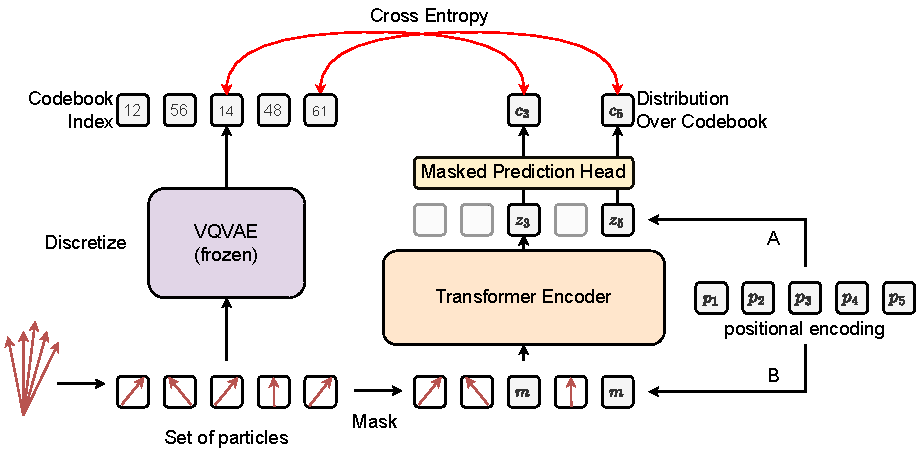
\includegraphics[width=0.99\linewidth]{Figures/foundation_models/mpm1.pdf}
    \caption{
        The proposed model and training scheme for MPM.
        Jets are represented as a set of particles, and some are selected to be replaced by masked tokens and passed through a transformer encoder.
        Training aims to predict the discrete token identity, defined by the output of a pre-trained VQVAE, of the masked particles.
        Positional encoding can be used in the prediction head (A), or in the backbone inputs (B).
    }
    \label{fig:mpm1}
\end{figure}

\subsubsection{Making Tokens From Particles}
\label{subsec:vqvae}

An effective tokenization scheme is essential to evaluating the impact of using discretized particles for model input or recovery.
The most straightforward approach involves binning each feature into a finite set of ranges~\cite{JetGPT}.
We find that discretization via the K-Means algorithm~\cite{KMeans}, whereby fitted clusters are assigned indices used as targets for the backbone, proved to be more performant than binning.
Both of these methods however lack contextual information regarding particle features relative to the rest of the jet.

For a context-dependent tokenization scheme, we employed a Vector Quantized Variational Auto-Encoder (VQVAE)~\cite{VQVAE}.
A VQVAE is defined with a set number of codebook vectors.
An encoder maps inputs to latent vectors, which are projected onto the nearest codebook element and then decoded.
We use transformer as the VQVAE encoder which maps each particle to a single codebook element, conditioned on all other particles in the jet.

\subsubsection{Fine-Tuning}
\label{subsec:fine-tune}

Evaluating the utility of a pre-trained backbone requires suitable downstream tasks for benchmarking.
This work focuses on jet classification in various contexts, using a weighted pooling on the backbone output followed by a linear layer to match the number of jet classes.
Three strategies are examined for training a model for a downstream task:

\begin{itemize}
    \item \textbf{Fixed backbone}: The pre-trained backbone is frozen during the supervised task, with only the linear classification head updated. This tests the linear separability of fixed representations.
    \item \textbf{Fine-tuned}: Both the linear classification head and backbone model are fit to the downstream task, evaluating the utility of pre-training for initializing the model's function.
    \item \textbf{From scratch}: The backbone model is reinitialized with new weights and fit directly on the downstream task, providing a performance benchmark without pre-training influence.
\end{itemize}

\subsection{Data}
\label{sec:mpm_data}

MPM does not require labels and can be directly applied to experimental data.
However, due to the lack of readily accessible large open datasets of real jets (at the time of writing), we use MC simulations to develop the framework.
We ignore all truth labels during pre-training but use them to evaluate the model's performance on downstream tasks.

We use the publicly available JetClass dataset~\cite{JetClass} with 125 million jets across 10 classes (100M for training, 5M for validation, 20M for testing).
Jets in this dataset are fat jets, \Cref{sec:fat_jets}, comprising multiple quark or gluon jets overlapping due to highly boosted decays.
Each class represents jets captured when simulating specific decay chains, such as $H \rightarrow b\overline{b}$, and $t \rightarrow b \ell \nu$.
Events in JetClass are generated using \pythia~\cite{Pythia8}, with top, W, Z, and Higgs decays modelled with \madgraph~\cite{MadGraph}.
Detector simulation is performed using \delphes~\cite{Delphes} and is configured to match the CMS experiment.
Jets are reconstructed using calorimeter energy deposits with the anti-$k_T$ algorithm~\cite{AntiKt} with the radius parameter set to $R=0.8$.
Jets are selected to have roughly the same transverse momentum $\pt$ distribution across all classes, ranging from $500$ to $1000~\GeV$.
On average, each jet contains 50 particles, with a maximum of 120.

For our experiments, each particle is virtually massless and described by its transverse momentum $\pt$, pseudo-rapidity to jet axis $\Delta\eta$, and azimuthal angle to jet axis $\Delta\phi$.

\subsection{Model Architecture}

The same transformer encoder architecture is used as the backbone in all experiments.
Eight TE Blocks based on the Normformer architecture~\cite{Normformer} are used with a model dimension 1024, comprising a total of 40 million parameters.
Input particles are linearly embedded into this space.

After passing through the backbone, the output nodes are used in dedicated layers called \textit{heads}.
The pre-training head consists of a single MLP applied per node, followed by a softmax for classification or a linear layer for regression.
The fine-tuning classification head is a weighted average over all output dimensions, followed by another linear layer and softmax.

All models are trained with the AdamW~\cite{AdamW} optimizer using a learning rate of $10^{-4}$ and a weight decay of $0.01$.
Pre-training was performed over five epochs on the full JetClass dataset.
For supervised fine-tuning, all models were trained for up to 50 epochs with early-stopping enabled.
In both settings the learning rate was ramped up linearly from zero over 1000 steps and the norm of the gradients was clipped to 1.0.

In the tokenized settings, a codebook of size 512 was used for the VQVAE and 512 centroids for the K-Means.
For the masking strategy we set the mask rate $D_f=\sfrac{M}{N}$ to 0.3, meaning 30\% randomly selected particles in the jet were masked.

\subsubsection{VQVAE Training}

A VQVAE consists of an encoder $F$ and decoder $G$, a quantization layer $h$, and a codebook ${C}=\{c_i\}_{i=1}^m$ for vectors $c_i \in \mathbb{R}^n$ where $n$ is the latent space dimension.

The quantization layer $h: \mathbb{R}^n \times {C} \rightarrow c \in {C}$ acts on a latent vector by assigning it to the closest codebook element.
We use the euclidean norm as the distance measure.
The codebook $C$ will always be omitted from the arguments of the function $h$ in the following.
The output of a VQVAE is defined as,
\begin{align}
    \hat{x} & = G(h(F(\x))) \\
            & = G(h(\z_e))  \\
            & = G(\z_q),
\end{align}
for a given input $\x$.
The objective of a VQVAE is typically to minimize the reconstruction measure in the input space.
Gradients for this loss however can not be backpropagated to the encoder as the operation $h$ is not differentiable and have to be estimated using the straight-through estimator~\cite{StraightThrough}.
An extra commitment loss term is included to create an attractive force between the encodings $(z_e=F(x))$ and their corresponding codebook vectors $(z_q = h(z_e))$,
\begin{equation}
    \mathcal{L}_{cmt} = (1-\beta)d(z_e,\mathrm{sg}(z_q)) + \beta d(\mathrm{sg}(z_e),z_q),
\end{equation}
where $\mathrm{sg}$ is the stop gradient operator and $d$ is some distance measure which we take to be the euclidean norm.
We add this to the reconstruction loss with a relative weight of 10, and use a $\beta$ of 0.9.

Training a VQVAE~\cite{VQVAE} can be challenging.
One of the main issues is the collapse of the codebook, where all latent vectors are assigned to a single codebook element.
We employ several best practices to mitigate this issue~\cite{bettervqvae} via the library vqorch~\cite{VQTorch}.
We use a shared parameterization for the codebook elements, update the commitment loss only every four steps, a synchronized update rule with $\nu=2$, and a latent dimension of $n=16$.
The codebook elements are initialized using the K-Means clustering algorithm on the latent space of a randomly initialized model.
Specific codebook elements which have not been used for 100 consecutive steps are reinitialised.
Post-training, the codebook achieves approximately 80\% utilization.

The input nodes are each quantized and decoded separately, with the distance calculated on a per-node basis.
Therefore, a jet with $N$ constituent particles is assigned to $N$ codebook elements, each of dimension $16$.
Each of these codebook elements are decoded to $N$ vectors of the same dimension as the input nodes.
Using a transformer for the encoder and decoder networks ensures that the model is encoded and decoded conditional on all particles in the jet.
The encoder and decoder follow a similar structure to the backbone but with only four layers and a model dimension of $256$, and linear layers resize the inputs and outputs.

\subsection{Experiments}

The first set of experiments are conducted to test the model design strategies.
These experiments aim to understand the impact of tokenization on the inputs and targets features, examine the quality of tokens learned by the VQVAE, and test the effect of the positional encoding.
These are followed by experiments to evaluate the performance of the models on downstream classification tasks.
The tasks include:
\begin{itemize}
    \item In-distribution prediction, where predictions are made using the same classes seen in pre-training
    \item Out-of-distribution (OOD) prediction, where predictions are made using the classes not seen in pre-training
    \item Weakly supervised prediction, where a CWoLa style classifier is trained using noisy labels as described in \Cref{sec:drapes}
\end{itemize}
All experiments are repeated five times with different seeds, and the mean and standard deviation of the results are reported.

\subsubsection{Token Creation with a VQVAE}

To ensure that latent space codes sufficiently capture essential information about particles in a jet, we examine the quality of decoded jet properties after encoding and quantization in the VQVAE.
\Cref{fig:vq_vae} shows that the distributions of decoded jet transverse momentum and mass align well with the input distributions.
Despite the apparent overlap in goals between VQVAE and MPM models, VQVAEs primarily focus on data compression, while masked particle models infer missing information to understand a jet and thus face a more challenging task.

\begin{figure}[htp!]
    \centering
    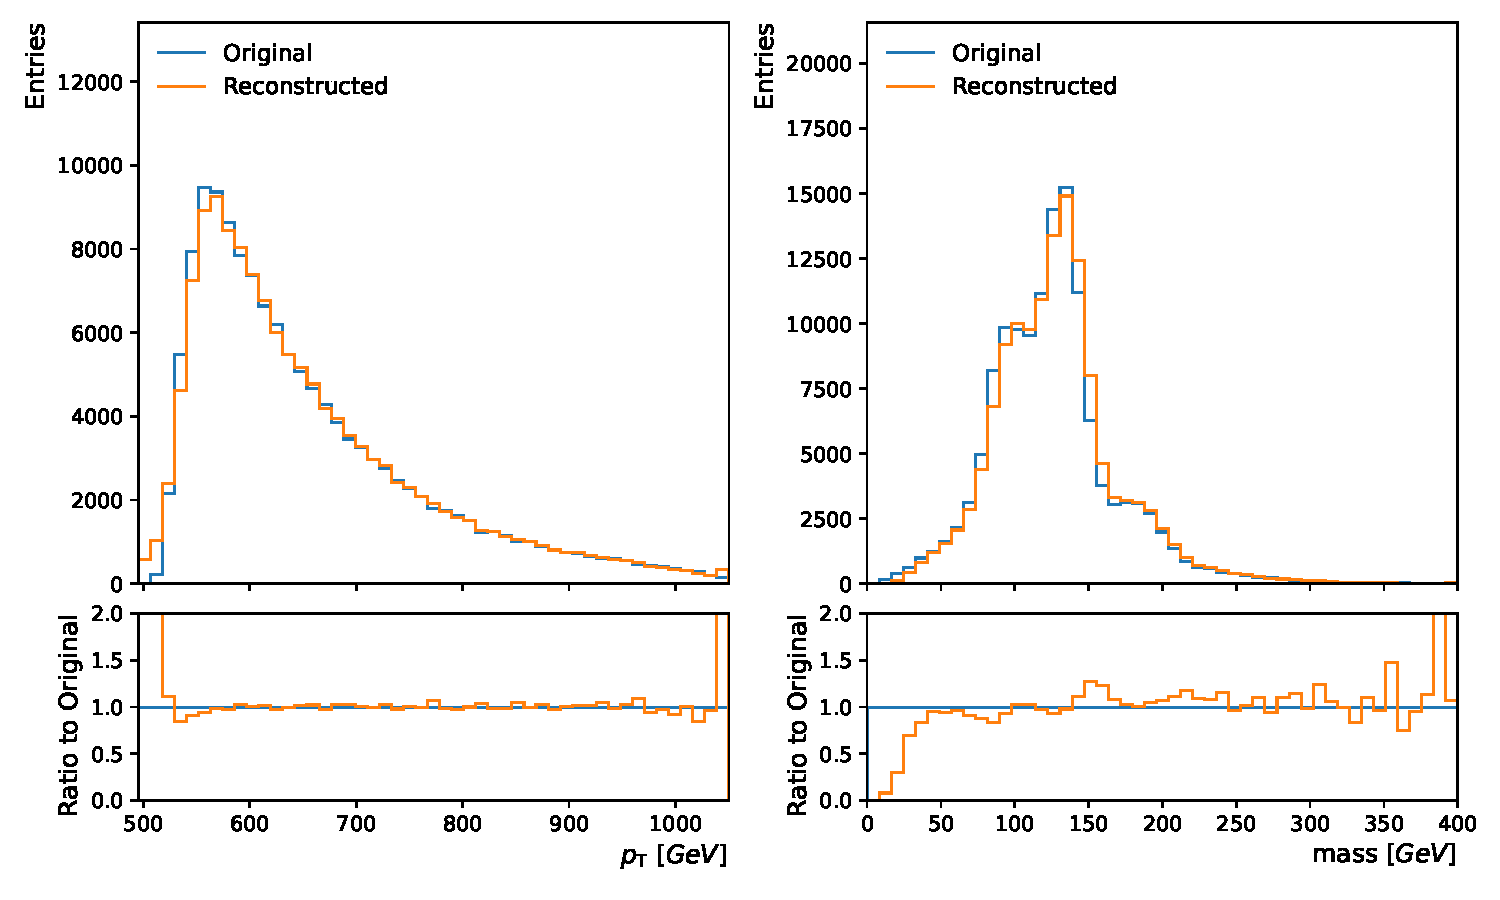
\includegraphics[width=0.8\textwidth]{Figures/foundation_models/mpm1/jet_high_img.pdf}
    \caption{
        \label{fig:vq_vae}
        The reconstruction of the jet mass and transverse momentum using the VQVAE.
    }
\end{figure}

\subsection{Discretization and Positional Encoding}

This section examines the pre-training configuration, focusing on the impact of positional encoding, input quantization, and target quantization.

The ordering settings considered include no ordering within the model, ordering at the backbone input, and ordering at the pre-training prediction head input.
Ordering is defined by decreasing particle transverse momentum, with the index in the sequence embedded using learned absolute positional encoding (APE).
We also test the impact of replacing the continuous features to the backbone with discrete tokens defined by either the VQVAE or K-Means clustering.
This is used for the input features, the target features, or both.
When a tokenized representation is used for the target, the model is trained using cross-entropy over the codebook indices. Otherwise, we use regression with mean squared error.

After pre-training we fix the backbone and train a linear classifier on the JetClass dataset.
The accuracies are quoted in \Cref{tab:pretraining_compare}.
Ordering solely in the model head demonstrates a clear advantage over ordering the backbone inputs or not ordering at all.
Input quantization negatively impacts model performance due to the information loss.
Using tokens from either the VQVAE or K-Means as classification targets is substantially better than regressing particle features as a prediction task, since regression offers only a point prediction of average particle properties under the posterior, which has limited predictive power for multi-modal posteriors.
Classification loss is more flexible, allowing for the prediction of the full posterior over tokens.
VQVAE tokens outperform K-Means tokens for classification, likely due to the VQVAE's complexity in capturing subtle details.
However, K-Means tokens perform reasonably well and may be a useful avenue for additional tests due to the ease of implementation compared to the VQVAE.

Following these results, all subsequent tests use a backbone with original continuous inputs, ordering in the prediction head for pre-training, and a classification loss using VQVAE tokens as targets in the pre-training.

\begin{table}[htp!]
    \centering
    \caption{Linear probe accuracy on the ten classes of JetClass using backbones with different pre-training strategies. The accuracy is averaged over five different runs with errors on the order of $0.01\%$.
    }
    \label{tab:pretraining_compare}
    \begin{tabular}{lllc}
        \toprule
        Inputs       & Targets        & APE           & Accuracy          \\
        \midrule
        \textbf{raw} & \textbf{VQVAE} & \textbf{head} & $\mathbf{56.8\%}$ \\
        original     & K-Means        & head          & $56.2\%$          \\
        original     & VQVAE          & none          & $54.1\%$          \\
        original     & VQVAE          & backbone      & $53.4\%$          \\
        VQVAE        & VQVAE          & head          & $51.1\%$          \\
        VQVAE        & K-Means        & head          & $49.3\%$          \\
        original     & original       & head          & $48.9\%$          \\
        original     & original       & backbone      & $46.3\%$          \\
        \bottomrule
    \end{tabular}
\end{table}

\subsubsection{In-Distribution Classification}

The utility of the backbone model for downstream tasks is first tested on in-context data by examining the accuracy of ten-class classification on a JetClass test sample.
We perform fine-tuning on the same dataset as with pre-training and then measure the results with respect to the holdout test set.
We modify the number of labelled samples used for fine-tuning to assess the data efficiency.

Figure ~\ref{fig:fine_tune_jetclass} shows that with labelled dataset sizes under 10k jets, pre-training offers a significant performance advantage over the supervised model trained from scratch.
This demonstrates the utility of the representation learned during pre-training for downstream tasks.
With a sufficiently large labelled dataset, the supervised model surpasses the fixed backbone model and matches the performance of the fine-tuned backbone model.
This is expected, as supervised learning on a large enough labelled dataset optimizes the model without pre-training.
Overall, pre-training provides a strong set of initial weights for fine-tuning on downstream tasks.

\begin{figure}[tp!]
    \centering
    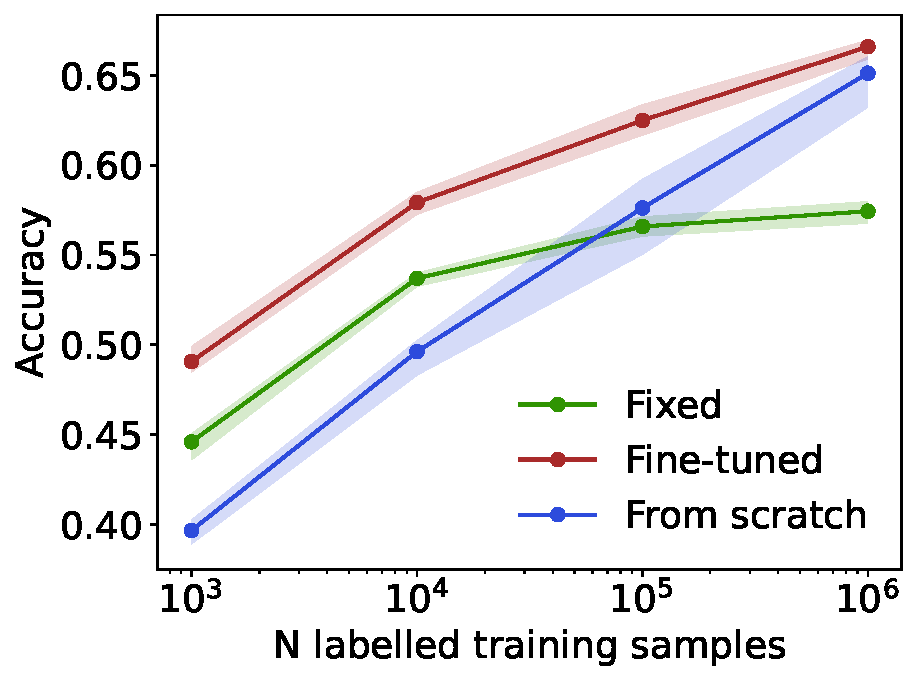
\includegraphics[width=0.5\textwidth]{Figures/foundation_models/mpm1/jc_corrected_pt_40_accuracy.pdf}
    \caption{
        Accuracy of training strategies as a function of the number of labelled samples. Uncertainty bands depict variability in five runs with different seeds.
        ``Fixed'' denotes models with frozen pre-trained weights; ``Fine-tuned'' denotes models with updated weights; ``From scratch'' denotes models with randomly initialized weights.
    }
    \label{fig:fine_tune_jetclass}
\end{figure}

\subsection{Out-of-Distribution Classification}

To test whether the pre-trained model learns features useful for tasks on data beyond those seen during pre-training, we perform an out-of-context test.
We pre-train on six of the classes in the dataset, those pertaining to Higgs, light quarks, and gluons, and fine-tune on four new classes containing top quarks and $W, Z$ decays.

The results in Fig.~\ref{fig:fine_tune_jetclass_ood} show that both pre-trained models, fixed and fine-tuned, outperform training from scratch.
This demonstrates that the representations learned during pre-training are useful for out-of-context classes.
With sufficient labelled data, the fully supervised model surpases both pre-trained models.

\begin{figure}[tp!]
    \centering
    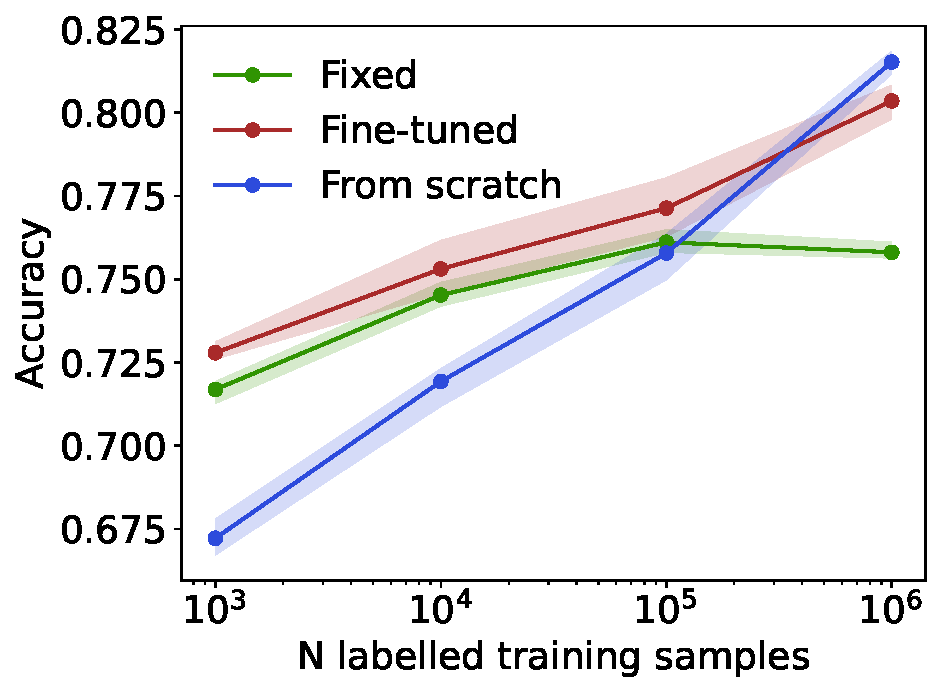
\includegraphics[width=0.5\columnwidth]{Figures/foundation_models/mpm1/jetclass_nc_two_40_accuracy.pdf}
    \caption{Accuracy of training strategies as a function of the number of labelled samples as measured on classes not seen during pre-training.
        Uncertainty bands depict variability in five runs with different seeds.
        ``Fixed'' denotes models with frozen pre-trained weights; ``Fine-tuned'' denotes models with updated weights; ``From scratch'' denotes models with randomly initialized weights.}
    \label{fig:fine_tune_jetclass_ood}
\end{figure}

\subsection{Weakly supervised classification}

Fine-tuning tasks are typically supervised and require labels.
Physics knowledge can enrich data in certain classes, providing training data with noisy labels.
These noisy labels can replace or complement fine-tuning with simulated data, leveraging pure labels in simulation and noisy labels in data.
This approach is useful for data-driven weakly supervised search strategies which use these noisy labels to construct a CWoLa classifier as described in \Cref{sec:drapes}.
However, CWoLa classification struggles with high-dimensional data when using large models like transformers on low-level set data.
Being able to improve their sensitivity via pre-training will make these methods viable for new physics searches.

To emulate the CWoLa setting, we take two samples of one class (QCD jets), each with one million events, and add $N$ samples of another class (top-quark initiated jets, or top jets) to one dataset.
A supervised classifier is then trained to discriminate between these datasets and evaluated on separating pure datasets of each class (QCD vs top jets).
In \Cref{fig:lp_ws}, significance improvement (SIC) is shown as the ratio of significance before and after applying a 0.5 threshold on the classifier output.
Significance is defined as the number of signal class events divided by the square root of the number of background class events passing the threshold.
The pre-trained backbone significantly improves the model's performance, even when only the linear head is fine-tuned.

\begin{figure}[htp!]
    \centering
    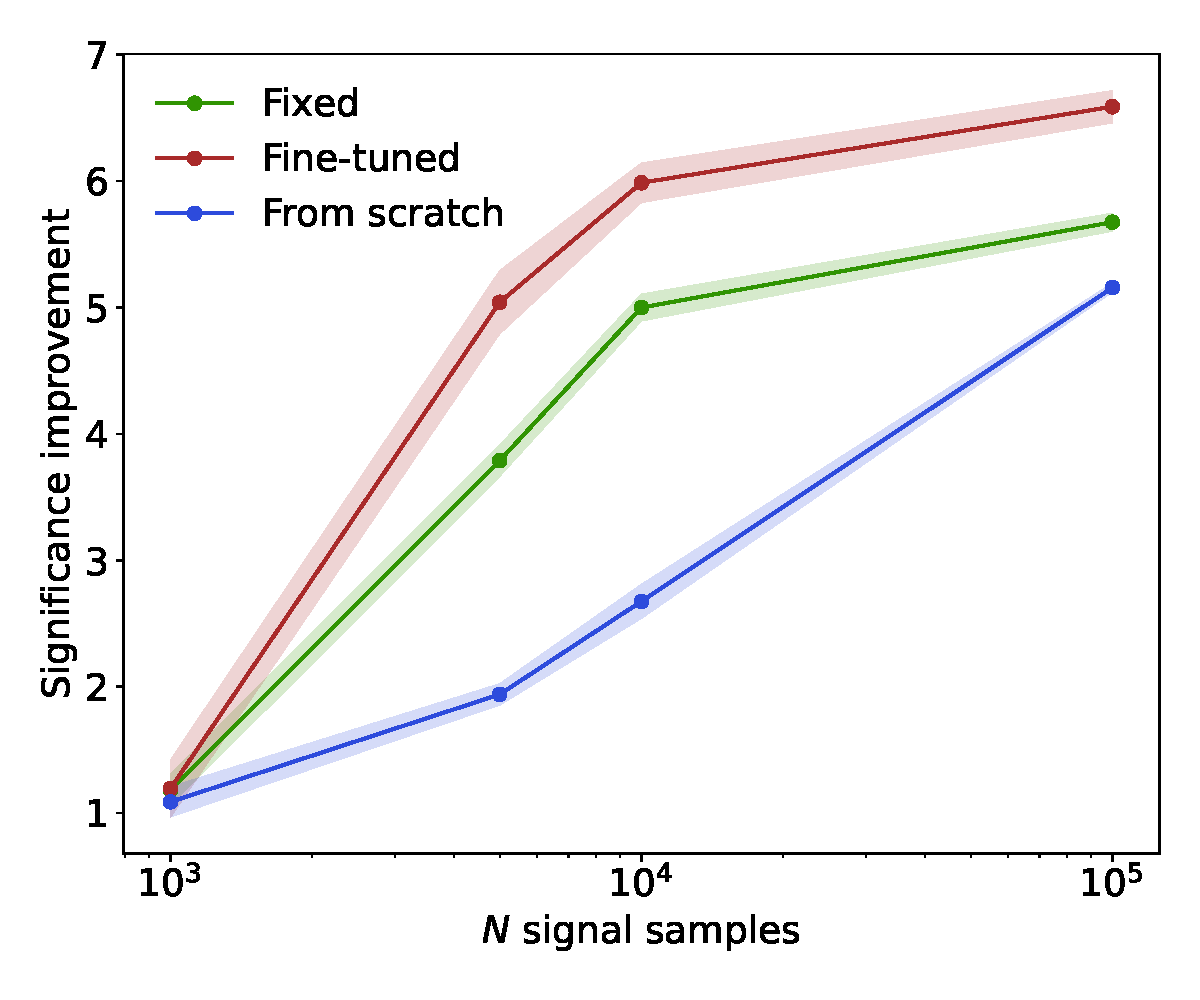
\includegraphics[width=0.5\columnwidth]{Figures/foundation_models/mpm1/cwola_40M_0.pdf}
    \caption{
        Models trained with weak supervision to classify datasets of different label proportions.
        A dataset of one million QCD jets is compared to a dataset with one million QCD jets plus $N$ top jets. Uncertainty bands depict variability in five runs with different seeds.
        ``Fixed'' denotes models with frozen pre-trained weights; ``Fine-tuned'' denotes models with updated weights; ``From scratch'' denotes models with randomly initialized weights.}
    \label{fig:lp_ws}
\end{figure}

\subsection{Conclusion}

We propose the masked particle modelling strategy for pre-training models on unordered sets of inputs, demonstrating its utility in the context of classifying jets.
This approach adapts masking strategies from NLP and CV to continuous, unordered particle features.
Pre-training with masked particle modelling allows fine-tuned models to perform well on downstream tasks, even with small datasets.
Initial results are promising, indicating that larger pre-training datasets and models could address domain adaptation challenges.
However, the model trained from scratch can surpass the pre-trained model with sufficient labelled data, indicating an inefficiency in the fine-tuning process.

\section{Improved Masked Particle Modelling}

In the previous section we found that a VQVAE leads to a more performant FM than direct regression.
We argued that this was primarily due to two reasons:
\begin{itemize}
    \item The VQVAE latent space is semantically rich, containing high-level abstractions; giving the MPM encoder a more informative target to learn from (this is also the justification used in BEiT~\cite{BEIT}).
    \item By changing from a regression to a classification task, the backbone is taught the full conditional posterior distribution rather than just seeking the mean.
\end{itemize}

However, producing the VQVAE requires an additional training step in the pipeline. VQVAEs are notoriously unstable and hard to train.
Furthermore, the aforementioned quantization leads to a loss of information.

In this follow-up study we make the following advancements:
\begin{itemize}
    \item We propose an improved MPM training paradigm, named MPMv2, by enhancing model architecture and addressing existing inefficiencies. We also expand the particle attributes to provide a more detailed representation.
    \item We provide a detailed study of alternative reconstruction tasks for MPMv2 pre-training, ones that replace the costly VQVAE-derived targets.
    \item We provide a new test bed for pre-trained models that include a wider set of downstream tasks commonly encountered in jet physics.
\end{itemize}
From henceforth, we refer to the original MPM method as MPMv1.

\subsection{Data}

We reuse the JetClass dataset~\cite{JetClass} but also introduce a new dataset, which we label BTag~\cite{btag}.
The BTag~\cite{btag} dataset contains 3 million jets differentiated by their flavour: light, charm, or bottom.

Events are generated using \pythia~\cite{Pythia8}, which also models parton showering and hadronization, and detector response is simulated using \delphes~\cite{Delphes}.
The BTag dataset is different from JetClass in several ways.
They are not large-radius or fat jets but are reconstructed using the anti-$k_T$ algorithm with a radius parameter of $R=0.4$.
The jets are only required to have $\pt \geq 20~\GeV$, and detector simulation is configured to match the ATLAS experiment instead of CMS.
The final significant difference is that BTag only stores charged particles; thus, they have a much lower cardinality, with a maximum of 15 constituents per jet.

We utilize JetClass exclusively for model pre-training, followed by fine-tuning and evaluation on both datasets.
The discrepancies between these datasets reflect the realistic variations in particle physics jet definitions across different experimental settings.
Targeted kinematic ranges, reconstruction parameters (e.g., anti-kt radius), and object selection vary significantly based on specific physics analyses and are meticulously tuned by experts.
These differences provide an opportunity to assess the backbone's generalizability to new downstream tasks and an OOD dataset that is further removed than the class separation we saw in MPMv1.

We also expand the input features to commonly reconstructed attributes beyond $\pt$, $\Delta\eta$, and $\Delta\phi$.
Charged constituents leave tracks in the detector, so we include the lifetime signed longitudinal and transverse impact parameters ($d_0$, $z_0$) as well as their reconstruction uncertainties ($\sigma(d_0)$, $\sigma(z_0)$), matching the features used in \Cref{ch:spice}
Neutral particles do not leave tracks, so these features are zero-padded.
These 7 variables form the continuous features of the particle, \xc.
Also included is the particle identity (ID) \xid, a one-hot encoded vector that categorizes both the particle type and charge into 8 independent classes.
Each particle is therefore represented by a vector of 8 features, 7 continuous and one categorical, $\mathcal{X} = \{\x_i=(\xc_i, \xid_i)\}_{i=1}^N$, as shown in \Cref{tab:mpm2_inputs}.
The distributions for these features in the two datasets are shown in \Cref{fig:mpm2_features}.

\begin{table}[ht]
    \centering
    \caption{The features used to describe each jet constituent.}
    \label{tab:mpm2_inputs}
    \begin{tabular}[t]{lr}
        \toprule
        \multicolumn{2}{c}{Continuous features \xc}   \\
        transverse momentum           & $\pt$         \\
        pseudorapidity to jet axis    & $\Delta \eta$ \\
        azimuthal angle to jet axis   & $\Delta \phi$ \\
        transverse impact parameter   & $d_0$         \\
        longitudinal impact parameter & $z_0$         \\
        uncertainty on $d_0$          & $\sigma(d_0)$ \\
        uncertainty on $z_0$          & $\sigma(Z_0)$ \\
        \midrule
        \multicolumn{2}{c}{Particle type \xid}        \\
        photon                        & 0             \\
        negative hadron               & 1             \\
        neutral hadron                & 2             \\
        positive hadron               & 3             \\
        electron                      & 4             \\
        positron                      & 5             \\
        muon                          & 6             \\
        antimuon                      & 7             \\
        \bottomrule
    \end{tabular}
\end{table}

\begin{figure}[h]
    \centering
    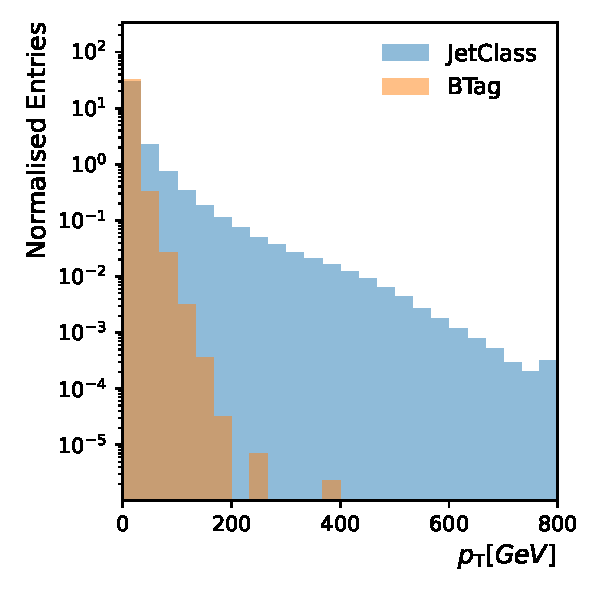
\includegraphics[width=0.32\linewidth]{Figures/foundation_models/mpm2/data/pt.pdf}
    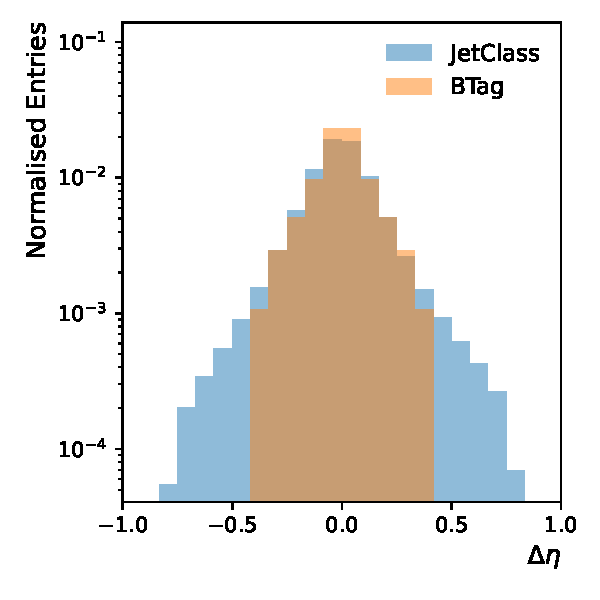
\includegraphics[width=0.32\linewidth]{Figures/foundation_models/mpm2/data/deta.pdf}
    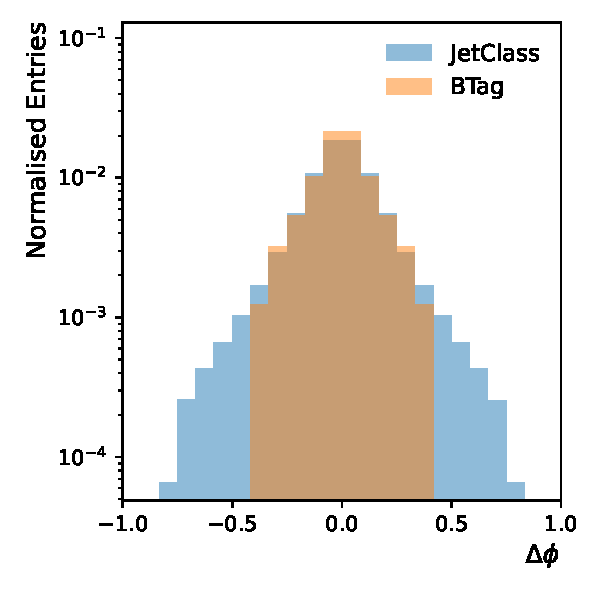
\includegraphics[width=0.32\linewidth]{Figures/foundation_models/mpm2/data/dphi.pdf}
    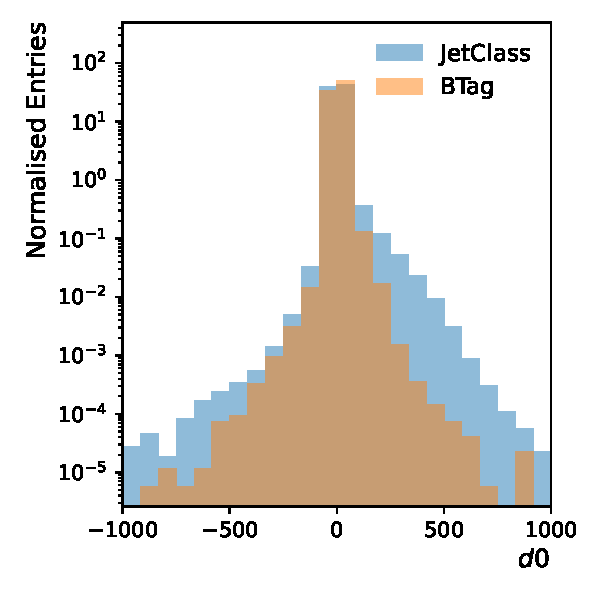
\includegraphics[width=0.32\linewidth]{Figures/foundation_models/mpm2/data/d0val.pdf}
    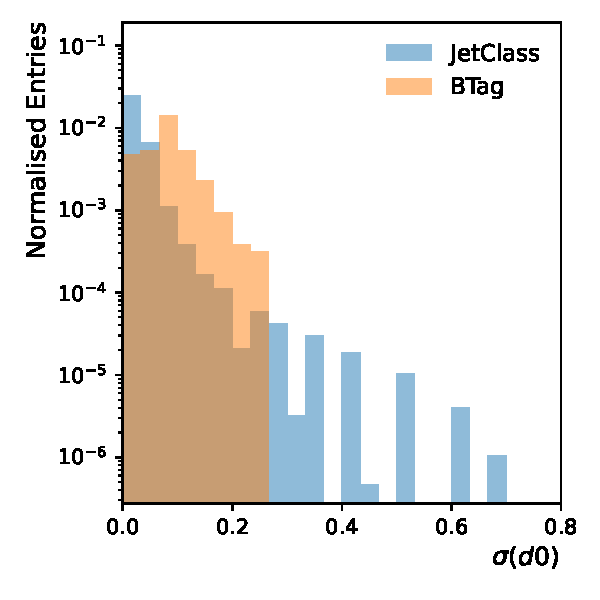
\includegraphics[width=0.32\linewidth]{Figures/foundation_models/mpm2/data/d0err.pdf}
    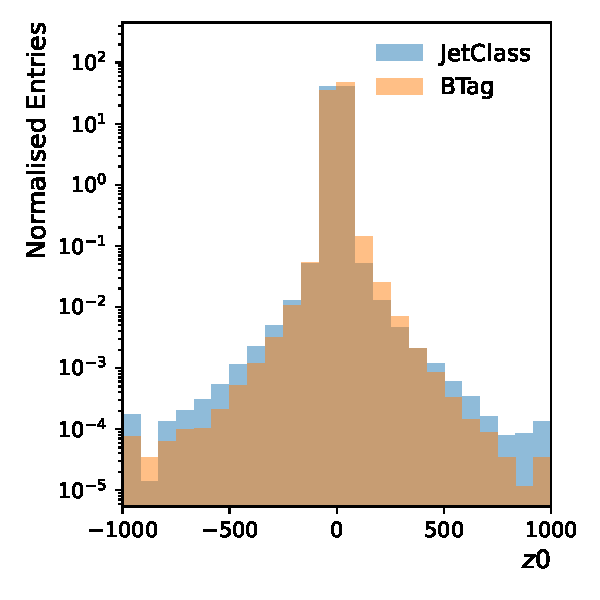
\includegraphics[width=0.32\linewidth]{Figures/foundation_models/mpm2/data/dzval.pdf}
    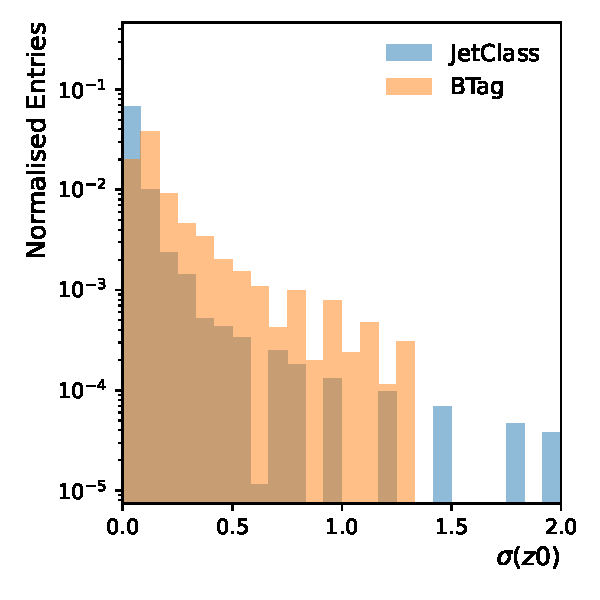
\includegraphics[width=0.32\linewidth]{Figures/foundation_models/mpm2/data/dzerr.pdf}
    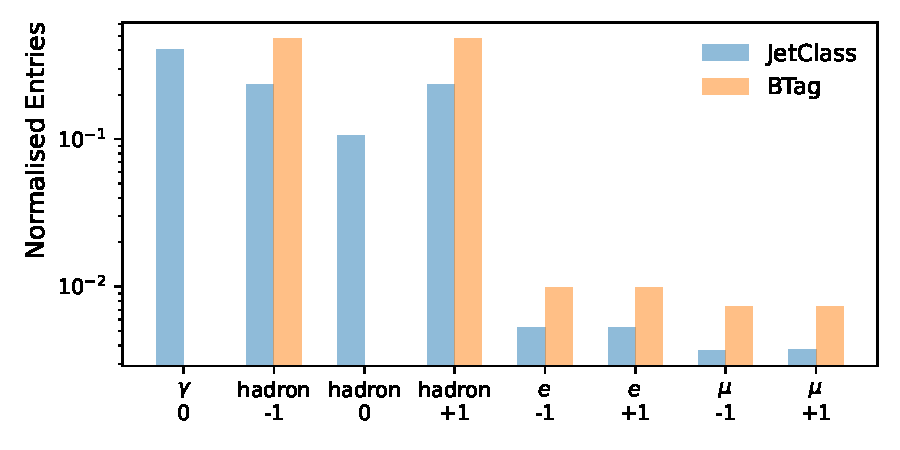
\includegraphics[width=0.64\linewidth]{Figures/foundation_models/mpm2/data/csts_id.pdf}
    \caption{The distributions of the particle features for the two datasets. The final plot shows the distributions of the particle types \xid for the two datasets.}
    \label{fig:mpm2_features}
\end{figure}

\subsection{Overview of Methods}

In framing MPMv1 as a DAE, the input jet $\mathcal{X}$, its latent projection $\mathcal{Z}$, and the decoder output $\mathcal{D}$ are all sets; thus, all mappings between them must be permutation equivariant.
A transformer acts as the encoder, and a multi-layer perceptron (MLP) acts as the decoder, applied separately per set element.
A consequence of having no PE is that the encoder's outputs corresponding to masked inputs are duplicates, so we are forced to add APE to $\mathcal{Z}$ to break this degeneracy for reconstruction while keeping the encoder equivariant.
Each element in $\mathcal{D}$ is then used in a tokenized reconstruction task, where it is compared to the corresponding element of the same jet passed through the encoder of a VQVAE.

For MPMv2, we propose removing the masked tokens from the input set, reintroducing them only during decoding, resulting in $\mathcal{Z}$ having a lower cardinality than both $\mathcal{X}$ and $\mathcal{D}$.
The masked tokens are identical in each sublayer of the decoder, effectively adding nothing to the message-passing operations.
This shifts from a model akin to BERT~\cite{BERT} to one similar to MAE~\cite{MAE}.
As such, we also experiment with expanding the decoder to a transformer, designed similarly to the backbone, albeit much smaller.

With a message-passing decoder, APE in the latent space provides too much information, trivializing the reconstruction task.
We only provide APE between the masked elements, not the full jet.
This can be parameterized by a unique mask token based on the \pt~order of the dropped constituents with respect to each other only.

The loss function is derived by comparing $\mathcal{X}$ and $\mathcal{D}$ across various \textit{reconstruction tasks}.
The key differences between MPMv2 and a direct MAE re-implementation include using multiple reconstruction tasks for different feature groups and positional encoding only for the dropped set.

\begin{figure}[t!]
    \centering
    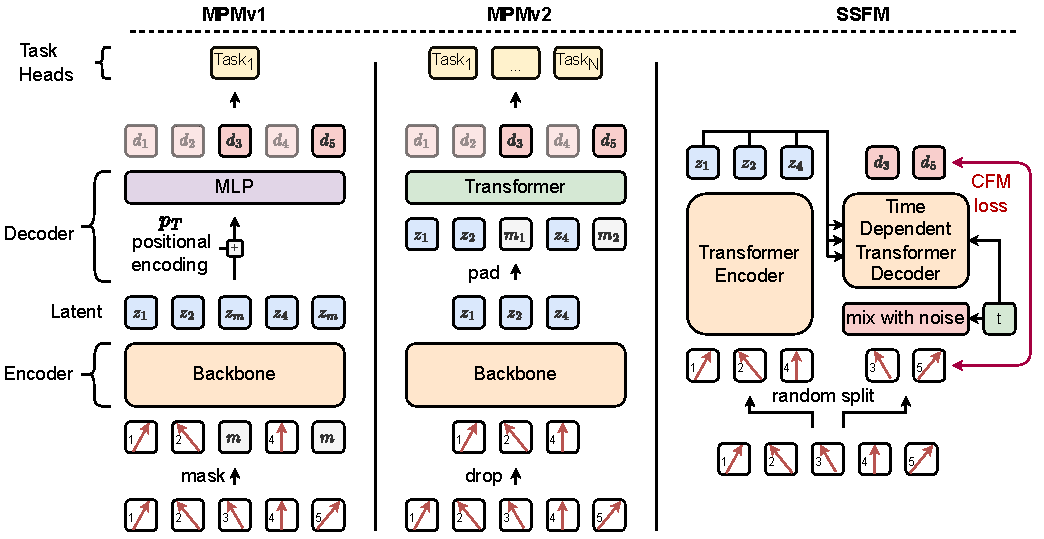
\includegraphics[width=\textwidth]{Figures/foundation_models/mpm2/FlowBert.drawio.pdf}
    \caption{(left) The original MPMv1 encoder-decoder setup compared to the new MPMv2 model (middle). The new model includes multiple reconstruction tasks, swaps the MLP decoder for a transformer, and only encodes the reduced set. (right) The Set-to-set Flow-Matching which jointly generates the dropped elements of the set using the surviving elements.
        \label{fig:models}
    }
\end{figure}

\subsection{Reconstruction Tasks}
\label{sec:recovery}

MPMv1 only uses a single VQVAE-derived reconstruction task, whereas MPMv2 combines multiple tasks to recover the continuous and categorical features separately.
Each task adds extra learnable layers (task head) and contributes to the total pre-training loss.
Each of these losses is applied per particle and only calculated for those which were masked/dropped.
We explore one task specifically for the categorical feature (\xid) and five options for the continuous features (\xc) and

\begin{itemize}
    \item Particle Identification: This is to recover the particle type \xid of the dropped constituent framed as a standard classification problem, so we use a linear layer for the task head and the cross-entropy loss function.
    \item Direct Regression: While we previously found direct regression insufficient for pre-training, we believe it is worth revisiting owing to the much more powerful decoder.
          We use a linear layer and find the best results using the L1-loss to recover the particles' continuous features.
    \item VQVAE Tokenized Classification: This is the method described in the previous section, whereby a frozen VQVAE is used to construct the target indices. We retrain the VQVAE for the expanded set of continuous.
    \item K-Means Tokenized Classification: We achieved similar results with the K-Means centroids as with the VQVAE tokens in the previous section. However, we can further optimize pre-training on K-Means targets by increasing the number of centroids to 16384.
          Like the other tasks, we use a single linear layer to map to this space and cross-entropy loss function.
    \item Conditional Normalizing Flow (CNF): If the strength of the tokenized form of reconstruction over regression is in learning the full posterior distribution $p(\xc_i|d_i)$, we can reproduce this using a generative model without needing to reframe the task as classification. The loss is the standard negative log-likelihood one uses for NFs.
    \item Conditional Flow Matching (CFM): Continuing with the idea of using PGM to conditionally generate the dropped continuous features given the surviving ones, we use a diffusion model via the CFM framework described in \Cref{sec:cfm}. We use the loss from \Cref{eq:linear_cfm_loss}.
\end{itemize}

\subsection{Set-to-Set Flow Matching}

We investigate the set-to-set flow-matching model (SSFM), shown in \Cref{fig:models}, which uses a time-dependent transformer decoder to generate constituents from latent nodes.
The approach is similar to the diffusion-masked autoencoder from CV~\cite{diffmae}.
During the masking the input set $\mathcal{X}$ is split into a reduced set $\mathcal{S}$ of size $M$ and its complement $\mathcal{T}$.
The reduced set passes through the encoder to obtain the latent set $\mathcal{Z}$, which is then used in the decoder's cross-attention layers, which trained as a set-CFM model to generate $\mathcal{T}$.

The training task of denoising prevents any degeneracy, eliminating the need for APE or mask tokens.
Furthermore, adjusting the masking rate $D_f = \frac{M}{N}$ controls fraction of the jet which is generated by the diffusion model.
When $D_f=1.0$, the decoder functions as a full generative model.
Our pre-training setup facilitates the creation of a backbone for embedding, as with MPM, as well as a decoder which could be used as a generative model, similar to those described in \Cref{ch:jet_generation}.
During training, sampling $D_f \sim \mathcal{U}(0.2, 1.0)$ balances these objectives.

\subsection{Model Architecture}

We propose several changes to the MPMv1 model.
We switched from the Normformer architecture to a more standard pre-norm encoder with 8 layers, each with a 512-embedding dimension.
We employ eight heads for multi-headed self-attention layers, feedforward network dimension multipliers of $\times2$, and SwiGLU activations~\cite{SwiGLU}.
LayerScale~\cite{GoingDeeper} is used for attention and dense residual updates.
The decoder used in the MPMv2 models uses the same layer types but is considerably smaller, with only four layers and a model dimension of 256.
In several of the experiments we use eight register tokens~\cite{VisionTransformersNeed} to store global information in the encoder.

Models are trained with the AdamW optimizer, a maximum learning rate of $1 \times 10^{-3}$, and weight decay of $1 \times 10^{-5}$.
The learning rate increases linearly for the first 50k steps and then decays exponentially with a 100k half-life.
Pre-training is conducted on the full JetClass training set with a batch size of 1000.

Each task head introduces new layers.
Most of these are simple affine layers to map the latent space to the target space.
The exceptions to this are the CNF and CFM tasks.
For the flow, we use six coupling layers with rational quadratic spline transformations, each containing a two-layer MLP with 128 hidden units.
The transformation is conditioned on the decoder outputs by concatenating them to the input of each MLP.
The CFM head uses a three-layer MLP with a hidden dimension of 256.
The inputs to this model are the partially noised targets ${\xc_i}(1 - t) + \z t$, the decoder outputs for the particle $d_i$, and the diffusion time $t$.

For the SSFM model, we use a transformer decoder with four layers, eight heads, and a model dimension of 256.
The layers have more parameters than the decoder used in MPMv2 due to the additional cross-attention layers.
A linear layer maps the latent space to the 256 for these cross-attention operations.
We use the method described in \textcite{DIT} for time injection.

\subsection{Experiments}
\label{sec:mpm2_experiments}

For these experiments we first test the impact of the new model design compared to the original MPMv1.
This is then followed by a full comparison of the different reconstruction pre-training strategies on a number of downstream tasks.

For the downstream tasks, we use the JetClass and BTag datasets.
Each backbone is pre-trained using one of the continuous feature reconstruction tasks (which it is named after) together with the particle ID task.
Pre-training is run for 1M steps, after which specific downstream task layers are appended to the encoder, and the model is fine-tuned.
All fine-tuning is run for 200k steps with a batch size of 500, allowing for early-stopping using a validation set.
We use a randomly initialized network, trained ``From Scratch'' as a baseline to highlight the performance provided by pre-training and repeat each experiment 5 times to estimate the run-to-run variance.

Fine-tuning performance is greatly enhanced using a specific scheduler for the backbone learning rate.
This scheduler is defined by two parameters: the number of frozen-steps and warmup-steps.
At the start of training, the backbone is frozen, which allows the new head to adapt.
Then, the backbone learning rate catches up to the head learning rate linearly over the warmup-steps.

\subsubsection{Ablation Studies}

To evaluate the proposed changes to the model, we use an in-distribution classification test on the JetClass dataset with a frozen backbone.
After pre-training for 200k steps, we freeze the encoder and add a classifier-head made from two class-attention layers~\cite{GoingDeeper}, which is then trained using cross-entropy loss for another 200k steps.
The regression, K-Means, and particle ID tasks are investigated, and the results of this ablation study are shown in~\Cref{tab:construction}.

Initially, the original training setup with a masking rate of $D_f=0.3$ was recreated.
We then tested updated transformer layers, added impact parameters to the input features, and included the particle ID feature and associated reconstruction task.
All of these changes improved the accuracy of the backbone, from $56.2\%$ to $74.0\%$ when using K-Means for the reconstruction task.
Changing the decoder to a transformer significantly increases classification accuracy, narrowing the gap between the K-Means and regression pre-training methods.
To verify the impact of the decoder change, we rerun the regression task without the impact parameters or particle ID task and found that it achieved an accuracy of 65.0\%, an increase of 9.5\%.

One additional advantage of adopting the MAE setup is achieving a 40\% reduction in GPU memory usage due to the reduced point cloud size passed to the encoder and the use of non-padded representations of the batch~\cite{FlashAttentionFastMemoryEfficient}.
The total inference time also improves by approximately 15\%.
Additionally, adding registers into the encoder~\cite{VisionTransformersNeed} prevents the transformer from overwriting elements in the set with global information, increasing performance with minimal computational cost.

Mask rate $D_f$ and decoder depth optimization results are shown in \Cref{fig:sweep}.
They both use the K-Means + ID setup, and the encoder depth sweep uses $D_f=30\%$ while the $D_F$ sweep uses a depth of 2.
The model is relatively robust to the mask rate; with values as high as $D_f=90\%$, it can still achieve an accuracy of over 80\%.
The optimal mask rate is determined to be $D_f=40\%$.
Increasing the decoder depth improves performance, but only four layers are tested due to computational constraints.

The final model is trained for 1M steps, with a mask rate of $D_f=40\%$ and a decoder depth of four.

\begin{table}[t]
    \centering
    \caption{The effects of the model redesign on the accuracy of a classifier head trained using the encoder outputs. All models except the final iteration are pre-trained using 200k steps, a 2-layer decoder, and $D_f=30\%$.
    }
    \label{tab:construction}
    \begin{tabular}[t]{lrlrl}
        \toprule
                                                                & \multicolumn{2}{l}{Regression} & \multicolumn{2}{l}{K-Means}                   \\
        \midrule
        MPMv1 using $(\pt, \eta, \phi)$                         & 48.9                           &                             & 56.2 &          \\
        + updated transformer layers                            & 55.5                           & \im{6.6}                    & 62.2 & \im{6.0} \\
        + impact parameter features                             & 62.2                           & \im{6.7}                    & 70.2 & \im{8.0} \\
        + constituent ID feature and ID reconstruction task     & 63.5                           & \im{1.3}                    & 74.0 & \im{3.8} \\
        + transformer as decoder (MAE)                          & 79.2                           & \im{15.7}                   & 81.4 & \im{7.4} \\
        + registers                                             & 80.4                           & \im{1.2}                    & 83.0 & \im{1.6} \\
        + longer train (1M steps) + deeper decoder + $D_f=40\%$ & 83.3                           & \im{2.0}                    & 84.0 & \im{1.0} \\
        \bottomrule
    \end{tabular}
\end{table}

\begin{figure}[htp!]
    \centering
    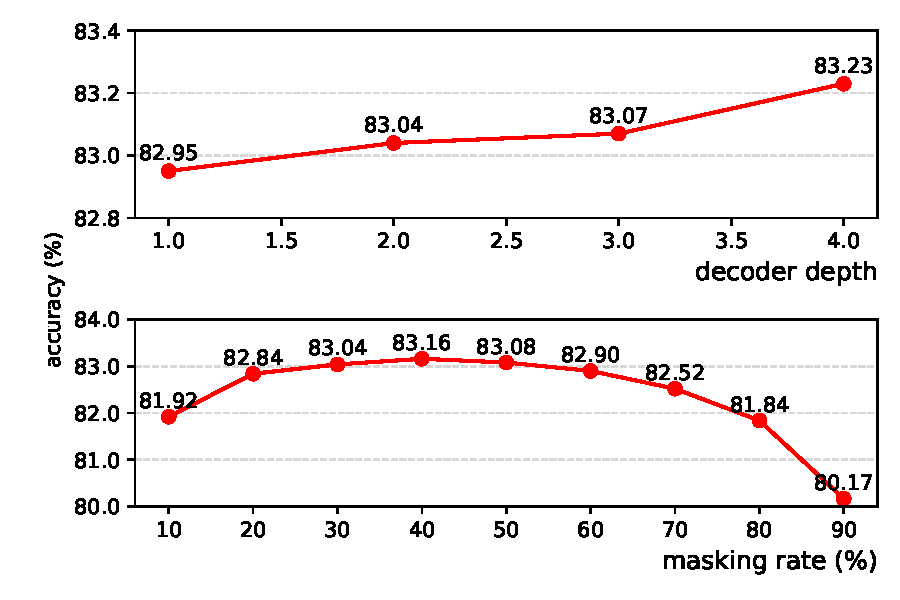
\includegraphics[width=0.7\linewidth]{Figures/foundation_models/mpm2/sweep.pdf}
    \caption{The effect of the decoder depth (top) and the mask rate (bottom) on the classification accuracy using the outputs produced by an MPMv2 backbone trained with the K-Means and ID tasks.}
    \label{fig:sweep}
\end{figure}

\subsubsection{In-Distribution Classification}

Classification is performed on the JetClass dataset using the classifier head as described in the ablation studies.
Data efficiency of the backbone is assessed by varying the number of jets used for supervised training from 1k to 100M, as shown in \Cref{fig:jetclass}.
For the 100M sample, all jets in the JetClass training set are used, but 200k steps limits the training to one epoch.
At each training set size, pre-trained backbones outperform the randomly initialized network, although the performance boost decreases with the number of jets.
At 100M jets, accuracy ranges between $85.0\%$ (regression) and $85.3\%$ (K-Means), compared to $84.3\%$ for random initialization.
The K-Means backbone excels with more data, while CNF and Regression backbones are more data-efficient.
The Flow backbone matches the performance of the random network with 1M jets using only 10k.
The state-of-the-art model ParT~\cite{ParticleTransformerJet} employs a similar transformer-based architecture, utilizing additional edge features and training with labels for 1M batches (520M jets), achieving an 86.1\% classification accuracy.

\subsubsection{Weakly Supervised Classification}

We emulate the CWoLa setting using the same methodology as in MPMv1 and use the same classifier head as the previous experiments.
In \Cref{fig:cwola}, we show the SIC at $r_b99\%$ for classifiers on a test set containing pure samples of QCD background and top signal.
The pre-trained backbones considerably outperform the benchmark, with the Regression backbone performing the best when only 500 top jets are present in the training set, resulting in a (SIC) of 8.18.

\begin{figure}[h!]
    \centering
    \begin{subfigure}{0.4\linewidth}
        \centering
        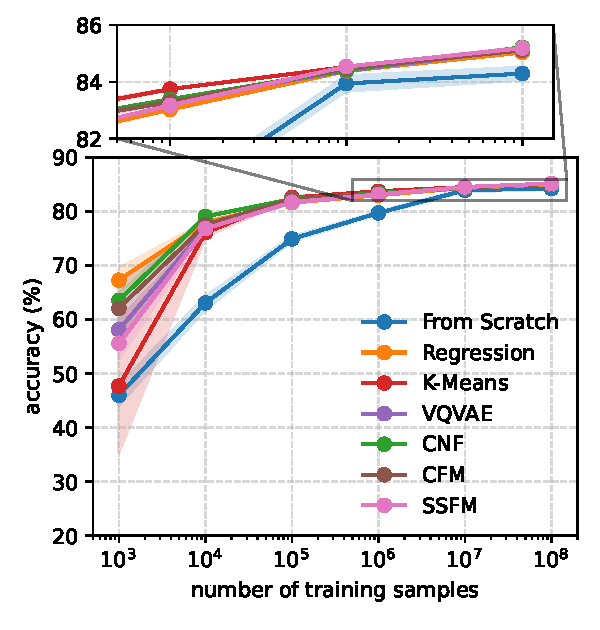
\includegraphics[width=\linewidth]{Figures/foundation_models/mpm2/final/jetclass_finetune.pdf}
        \caption{}
        \label{fig:jetclass}
    \end{subfigure}
    \begin{subfigure}[b]{0.4\textwidth}
        \centering
        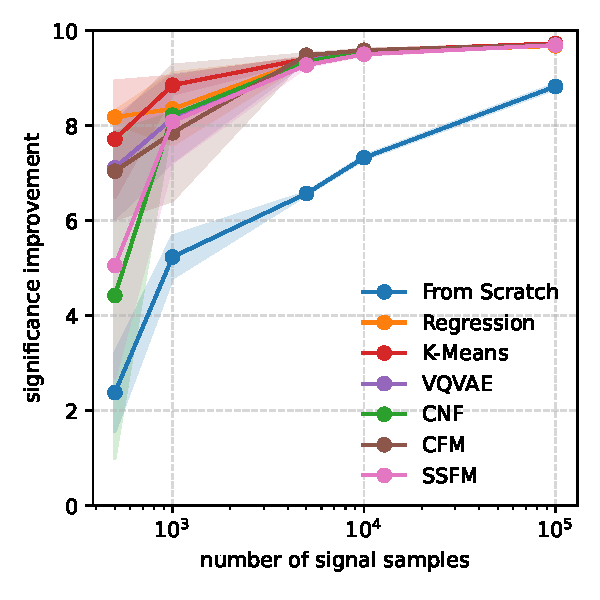
\includegraphics[width=\linewidth]{Figures/foundation_models/mpm2/final/cwola_finetune.pdf}
        \caption{}
        \label{fig:cwola}
    \end{subfigure}
    \caption{The in-distribution performance of the fine-tuned models on the JetClass dataset. \subref{fig:jetclass} shows the accuracy using standard supervised classification as a function of the dataset size. \subref{fig:cwola} shows the significance-improvement of the models trained in a CWoLa setting as a function of the number of signal samples in the dataset.}
    \label{fig:plot_A}
\end{figure}

\subsubsection{Out-of-Distribution Classification}

The performance of backbones in classifying the BTag dataset, which comprises lower-energy, narrower jets with a few charged particles, is tested.
As shown in \Cref{fig:btag}, the accuracy of the three-class classifier is presented as a function of the number of jets used for training.
All pre-trained backbones surpass the benchmark initialization, demonstrating the generalizability of the learned mappings beyond JetClass.
The CNF backbone achieves the highest performance in this task, but all pre-trained backbones converge at approximately 70\% accuracy with the maximum number of jets.

\subsubsection{Secondary Vertex Finding}

A track vertex denotes a common point from which reconstructed particle tracks originate, indicating an interaction or decay location.
Bottom and charm hadrons produced in the collision travel several millimetres beyond the interaction point before decaying, resulting in multiple vertices within the same jet.
These vertices are crucial for identifying heavy-flavor jets, as discussed in \Cref{ch:spice}.
Kaon decay also contributes additional vertices.
This task is recast as an edge classification problem, where pairs of tracks are classified as positive or negative.
This task is similar to instance segmentation in CV, where the goal is to segment the image into unique instances of different objects.
There are $N(N-1)/2$ unique pairs to evaluate for a jet with N tracks.

The additional layers for this task follow a twin-network approach~\cite{siamese}, where the probability that two tracks $x_i$ and $x_j$ originate from the same vertex is defined by $\sigma\left(G\left[|F\left(z_i\right)-F\left(z_j\right)|\right]\right)$, with $G$ and $F$ being MLPs, $z_i$ and $z_j$ as backbone outputs, and $\sigma$ as the sigmoid function.
The adjusted Rand index (ARI)~\cite{ari}, as used by \textcite{SecondaryVertexFinding}, is the designated performance metric.
The ARI is plotted against the number of secondary vertices in \Cref{fig:vtx}.
The backbone trained with the CNF task performs best, although all backbones surpass the benchmark.

\subsubsection{Heavy Track Identification}

Beyond grouping tracks by vertex, the task extends to identifying the vertex type associated with each track.
It resembles the track origin auxiliary task in \Cref{ch:spice}.
It also draws parallels with the semantic segmentation task in CV.
Tracks in the BTag dataset can be linked to a displaced $b$-quark decay, $c$-quark decay, or the primary vertex.
The task head is a straightforward three-layer MLP appended to the backbone, acting on each constituent independently.
Due to the heavily imbalanced class distributions, balanced accuracy is the preferred metric for distinguishing between pre-training methods.
As shown in \Cref{fig:trk}, balanced accuracy is plotted as a function of the number of tracks in each jet, with pre-trained backbones consistently outperforming the baselines.

\begin{figure}[h!]
    \centering
    \begin{subfigure}{0.32\linewidth}
        \centering
        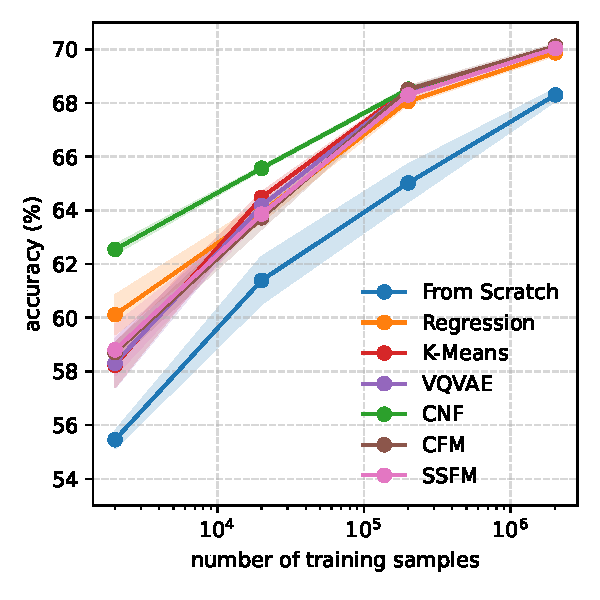
\includegraphics[width=\linewidth]{Figures/foundation_models/mpm2/final/btag_finetune.pdf}
        \caption{}
        \label{fig:btag}
    \end{subfigure}
    \begin{subfigure}[b]{0.32\textwidth}
        \centering
        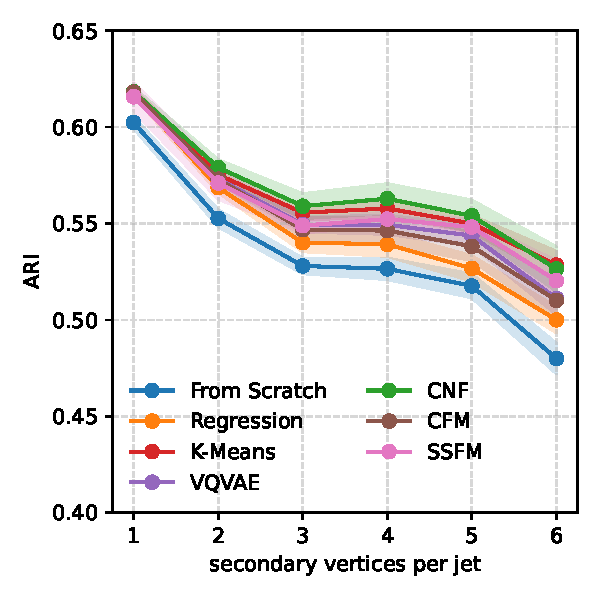
\includegraphics[width=\linewidth]{Figures/foundation_models/mpm2/final/vtx_finetune_ari.pdf}
        \caption{}
        \label{fig:vtx}
    \end{subfigure}
    \begin{subfigure}[b]{0.32\textwidth}
        \centering
        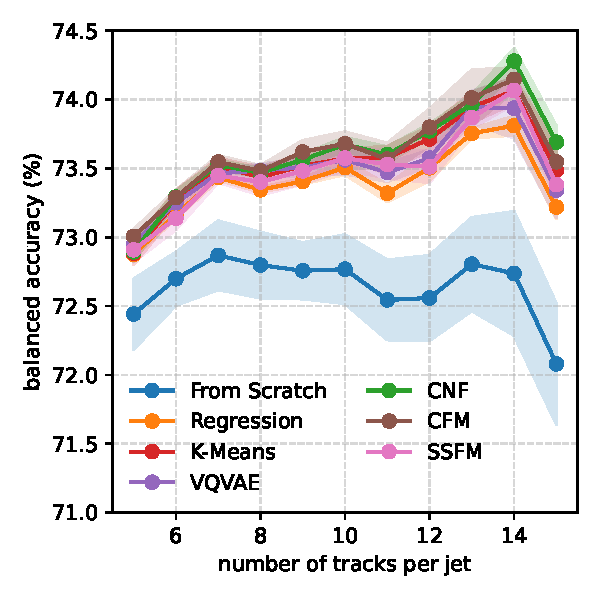
\includegraphics[width=\linewidth]{Figures/foundation_models/mpm2/final/trk_finetune.pdf}
        \caption{}
        \label{fig:trk}
    \end{subfigure}
    \caption{The performance of the fine-tuned models on the BTag dataset. \subref{fig:btag} shows the supervised jet classifier accuracy versus the number of samples used in fine-tuning.
        \subref{fig:vtx} shows the ARI score for the segmentation task versus the number of secondary vertices within each jet. \subref{fig:trk} shows the balanced accuracy for the track identification task as a function of the number of tracks in each jet.}
    \label{fig:plot_B}
\end{figure}

\section{Conclusion}
\label{sec:conclusion}

This study aims to build upon MPMv1's findings, in part by assessing the necessity of the costly tokenization step in pre-training.
Alternative reconstruction methods were explored, such as simpler tokenization through the K-Means algorithm and conditional generative models.
The new models significantly outperform an untrained backbone and the original MPMv1 in various tasks, including those involving out-of-distribution data. However, the differences between these pre-training strategies were minimal.
A key improvement was the implementation of a more powerful decoder.
Additionally, a novel pre-training method using set-to-set generation was introduced, proving competitive with MPMv2.
These findings suggest tokenization is not essential, which may have implications for other SSL models using VQVAE, such as \textcite{Omnijet}.

Despite the promising results, the self-supervised training strategies for particle physics jets face several limitations.
All experiments were conducted using the parametric \delphes fast simulation package, which does not fully replicate the complexity of real-world data.
The next significant step would be transitioning to real data and full simulations.
The approach is confined to jets and a few relevant downstream tasks, but another extension would be to move to full event-level data.
This would increase the expected set size from $O(100)$ to $O(1000)$, necessitating substantially more computation due to the transformer architecture and addressing these challenges is a key area for future work.
